\section{Results}\label{ch:results}

Using the test setup and mechanics described in section \ref{ch:testAndPerformance}, we conducted a experiment of four different scenarios. We wanted to see whether the hopping frequency would increase, when we increased the circumference of the track, evaluate the packet sent/loss ratio and measure the overall perception of data. The test results would indicate if our relaying algorithm, the implemented stop-and-wait ARQ protocol and distance measurements were correct and working. All results are gathered from the base station and can be found in appendix 10. To quickly iterate the parameters measured in the test runs: \\

\noindent \textbf{\textit{n} request packets sent ($p_1$):} Number of packets sent from the base station over the course of the test. These include retries due to ARQ timers expiring. Read this number as "times we have asked for data".

\noindent \textbf{\textit{n} packets relayed to node 1 ($p_2$):} Number of packets relayed to north relay station.

\noindent \textbf{\textit{n} packets relayed to node 2 ($p_3$):} Number of packets relayed to south relay station.

\noindent \textbf{\textit{n} ACK's received ($p_4$):} Number of acknowledgments received by the ARQ protocol. The closer this number is to the packets sent, the more stable the data link connection between our endpoints is.

\noindent \textbf{\textit{n} DATA's received ($p_5$):} Number of data packets received. Ideally, this should be close to the packets sent as well. If $p_5$<$p_1$, then $p_1$-$p_5$ request packets were not replied.

\noindent \textbf{\textit{n} packets not acknowledged in time ($p_6$):} Number of packets not acknowledged before the ARQ timer ran out. This is strongly related to the timers on the base station and heavily influenced by interference and signal noise. Also in our test set-up we tried to get as much data from the runner as possible, so timers were strict. \\

\noindent Table \ref{table:datascenarios1} and \ref{table:datascenarios2} show the final result of each completed scenario lasting 48 minutes each, which equals about 144 rounds with the train. Each minute we recorded parameters $p_1$ to $p_6$. All are initially set to zero. We decided not to change the RSSI threshold in each scenario.

\begin{table}[h]
	\centering
	\begin{tabular}{|l|l|l|l|} \hline
		Sn. & \pbox{10cm}{$p_1$} & \pbox{17cm}{$p_2$} & \pbox{17cm}{$p_3$} \\ \hline
		1 & 29148 & 4066 & 3512 \\ \hline
		2 & 29838 & 8115 & 8499 \\ \hline
		3 & 29258 & 3706 & 4021 \\ \hline
		4 & 30523 & 1232 & 8425 \\ \hline
	\end{tabular}
	\caption{Data from scenarios 1-4 for parameters 1-3.}
	\label{table:datascenarios1}
\end{table}

\begin{table}[h]
	\centering
	\begin{tabular}{|l|l|l|l|} \hline
		Sn. & \pbox{17cm}{$p_4$} & \pbox{17cm}{$p_5$} & \pbox{17cm}{$p_6$} \\ \hline
		1 & 22169 & 34167 & 20700 \\ \hline
		2 & 17880 & 23563 & 21111 \\ \hline
		3 & 21944 & 32830 & 21244 \\ \hline
		4 & 19137 & 28874 & 23188 \\ \hline
	\end{tabular}
	\caption{Data from scenarios 1-4 for parameters 4-6.}
	\label{table:datascenarios2}
\end{table}

\noindent As expected, the results vary depending on the track length and the channel used. When using a length of $56cm$ (scenario two and four), we see $p5$=<$p_1$, meaning the base station received the same or less data packets than requested. In scenario four they are even fairly close. If $p5$>$p_1$, it could be due to fading or missed timers. Also worth noting is the increased use of relays ($p_2$ and $p_3$) when the length is $56cm$. Changing channels between 11 and 4 seem to lower the difference between $p_1$ and $p_5$ as well.

\noindent Figure \ref{fig:noackreceived} shows the correlation between the number of ACK's received, $p_4$, at the base station per packet sent from it. These numbers should be close to each other. Scenario 2 received a large number of ACK's around the 24408 packet sent mark, perhaps due to deep fading.

\begin{figure}[h]
	\centering
	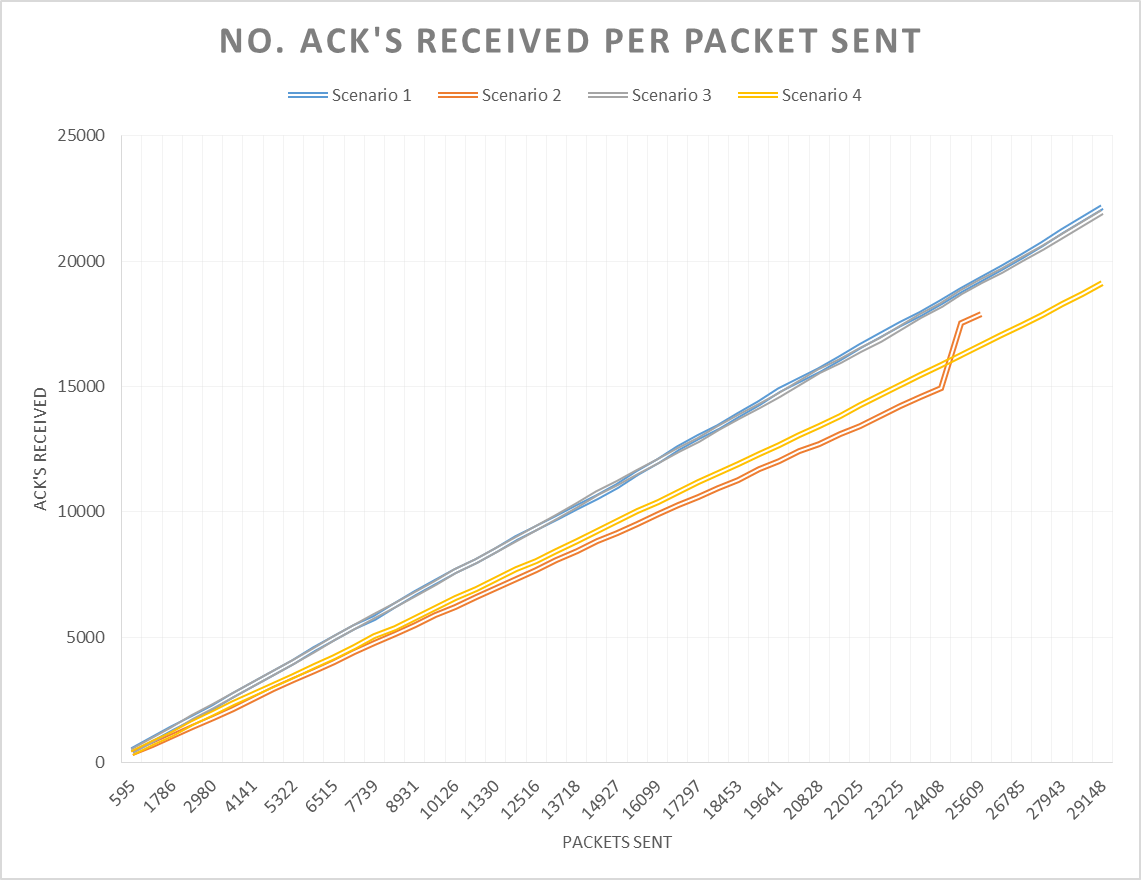
\includegraphics[width=1\linewidth]{results/NoAckReceived}
	\caption{No. ACK's received per packet sent.}
	\label{fig:noackreceived}
\end{figure}

\noindent Figure \ref{fig:nodatareceived} shows the number of data packets received, $p_5$, from the runner node either direct or via one of the relays per packet sent. Scenario 1 and 3 (length=$43.5cm$) follows each other slightly, however changing channel from 11 to 4 decrease the amount of additional packets received ($p_5$>$p_1$) when using length=$43.5cm$. Scenario 4 looks to be the most successful one, as the number of data packets received is close to the number of requests sent. We reflect on this at the end of results. Scenario 1 and 3 sees more data packets being received than requested. A probable cause is a packet not being acknowledged in time by the base station, so the runner will resend it, even though it might already have been received by the base station.

\begin{figure}[h]
	\centering
	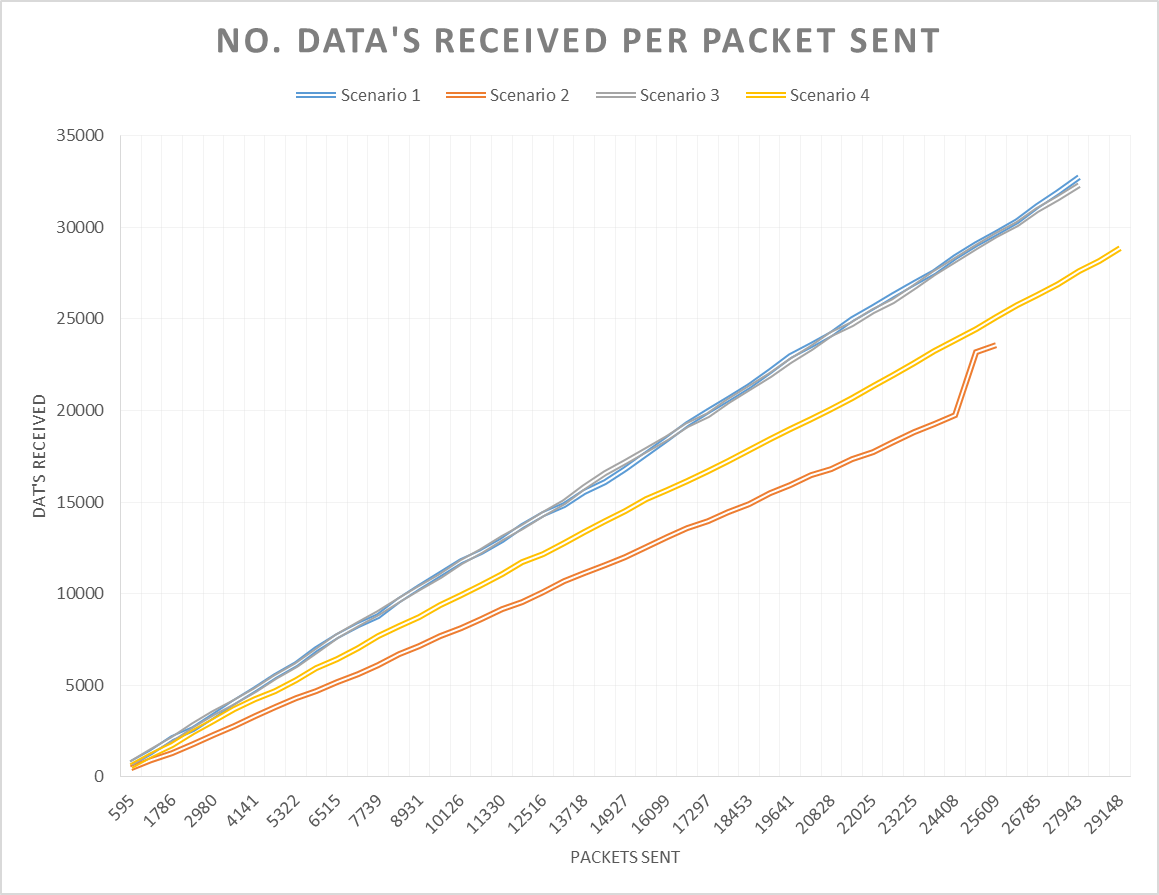
\includegraphics[width=1\linewidth]{results/NoDataReceived}
	\caption{No. DATA's received per packet sent.}
	\label{fig:nodatareceived}
\end{figure}

\noindent Figure \ref{fig:nopacketsrelayed} shows the number of data relayed to the north  and south relay station combined per packet sent. As expected, scenario 2 and 4 (length=$56cm$) relays more packages, now that the runner node will be out of reach from the base station for a longer period of time. It might even be that neither can reach the runner due to deep fading. Calculations made in Appendix 1 show the minimum theoretical packages send from the base station, which must be relayed at each of the track length. The total packages send from the base station ideally is 12280, the minimum relayed packages send from the the base station for scenario 1 and 3 are 2355 packages, and for scenario 2 and 4 the total packages send from the base station are 4961 packages. Both the number of relayed packages and the total number of packages send from the base station is flawed compared to theory and this will be further discussed in the discussion, but the inter scenario relative test results follows the theory well.

\begin{figure}[h]
	\centering
	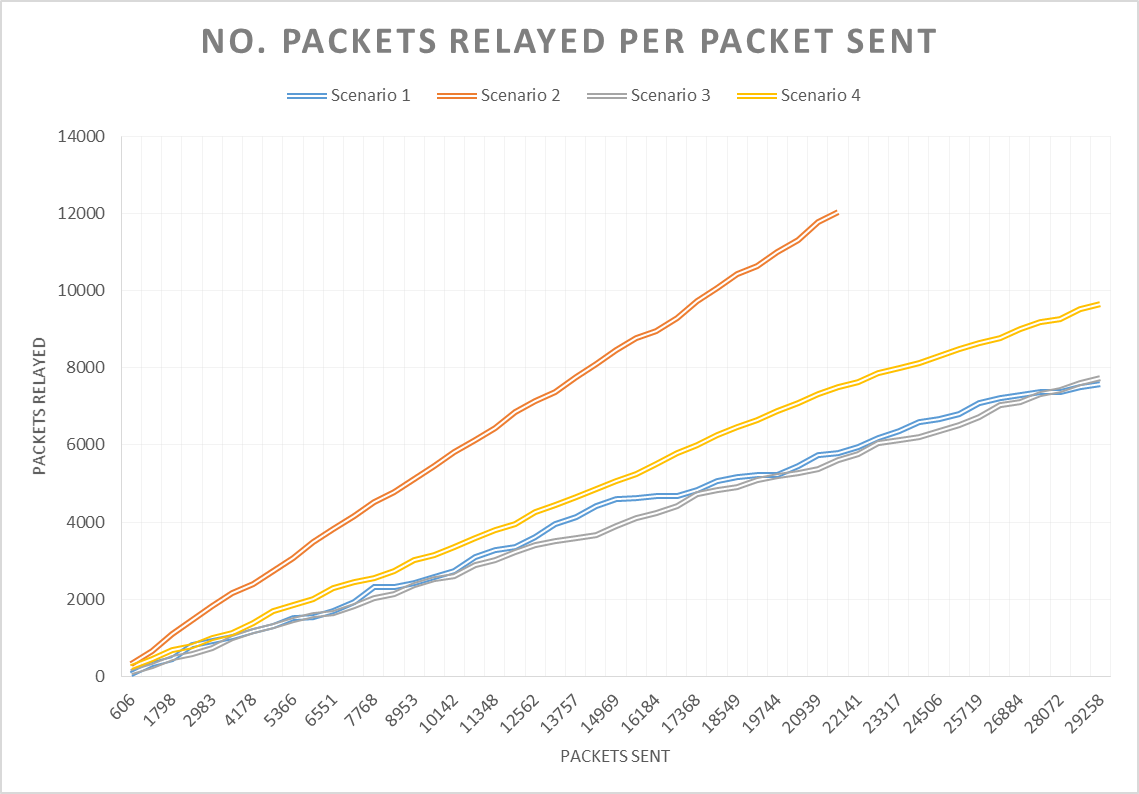
\includegraphics[width=1\linewidth]{results/NoPacketsRelayed}
	\caption{No. packets relayed per packet sent.}
	\label{fig:nopacketsrelayed}
\end{figure}

\noindent Figure \ref{fig:nopacketsnotackintime} shows the number of packets not acknowledged in time per packet sent. All scenarios follows each-other, which points to a systematically error either due to strict timers or fading issues. An error that channel or length does not seem to affect. We noticed during the live testing that more ARQ errors occurred when communicating directly rather than relaying. Figure \ref{fig:nopacketsrelayedscenario2} and \ref{fig:nopacketsrelayedscenario4} show how the two scenarios that relay the most packets (2 and 4) distribute the data among our two relay stations (north and south) per packet relayed. A bit strange is the sudden drop of packets relayed to the north station in scenario 4, figure  \ref{fig:nopacketsrelayedscenario4}. Probable reason is fading.

\begin{figure}[h]
	\centering
	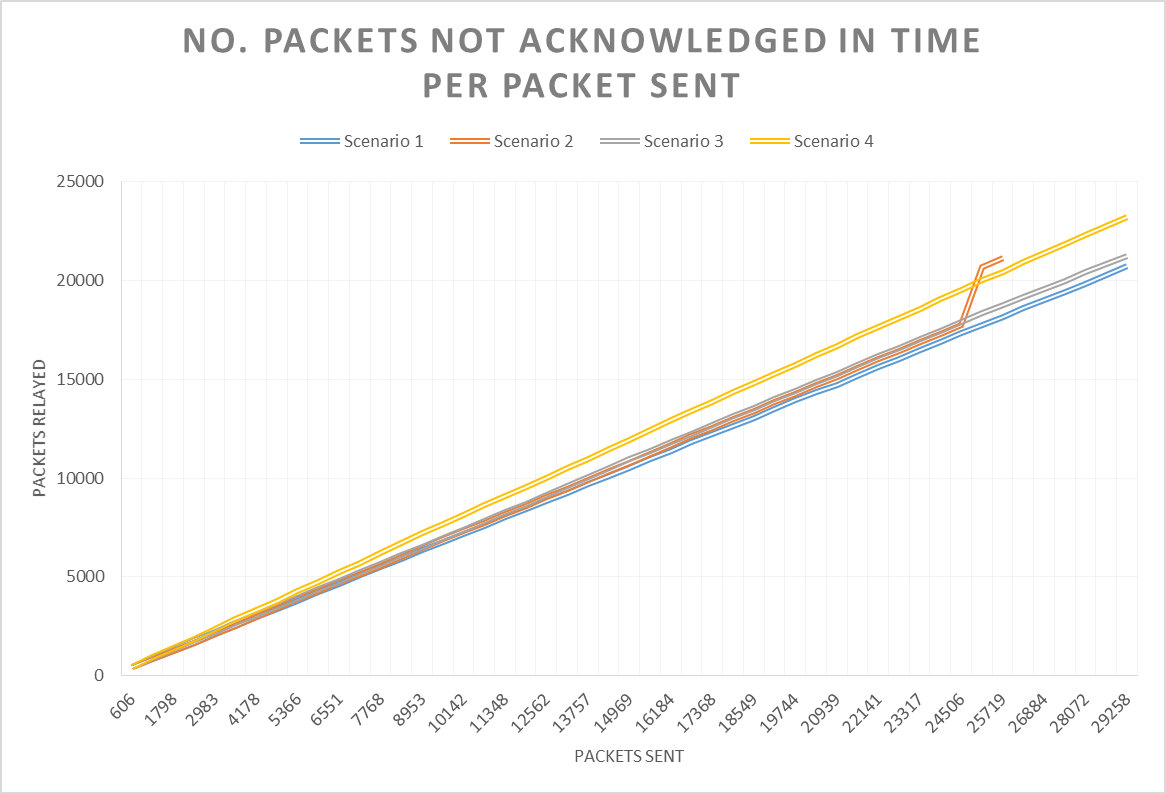
\includegraphics[width=1\linewidth]{results/NoPacketsNotACKInTime}
	\caption{No. packets not acknowledged in time.}
	\label{fig:nopacketsnotackintime}
\end{figure}

\begin{figure}[h]
	\centering
	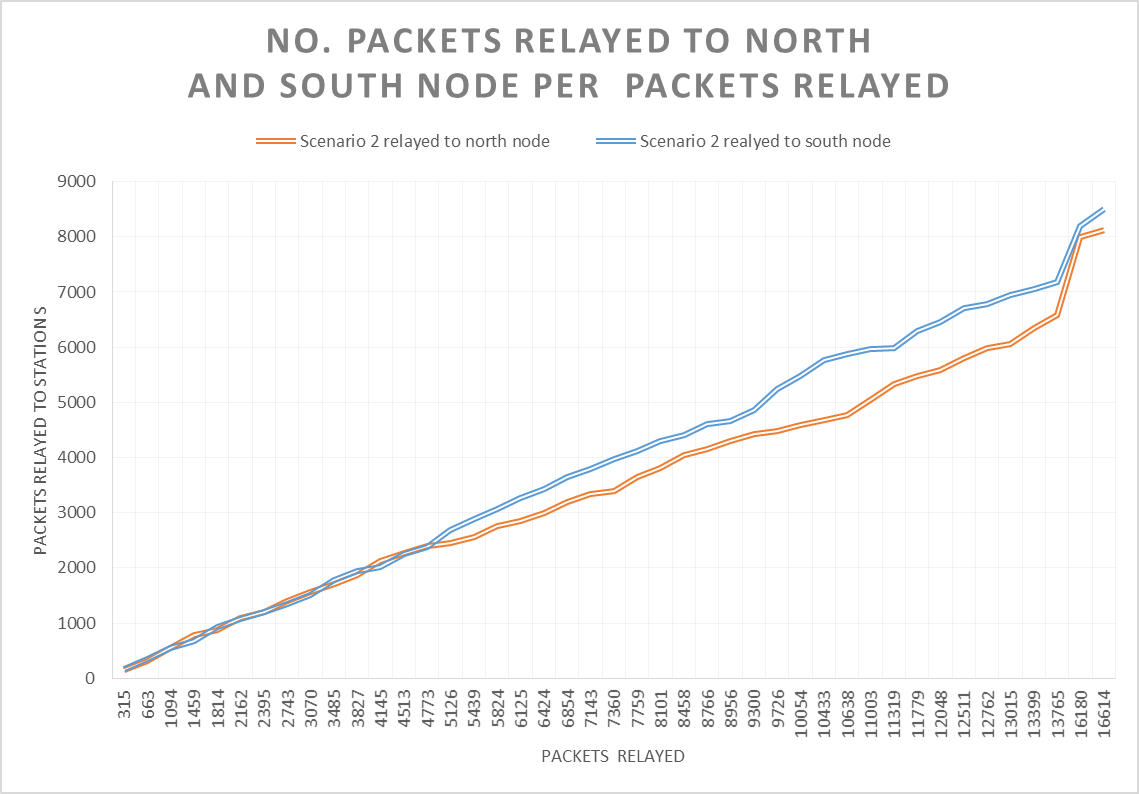
\includegraphics[width=1\linewidth]{results/NoPacketsRelayedScenario2}
	\caption{No. packets relayed to north and south node in scenario 2.}
	\label{fig:nopacketsrelayedscenario2}
\end{figure}

\begin{figure}[H]
	\centering
	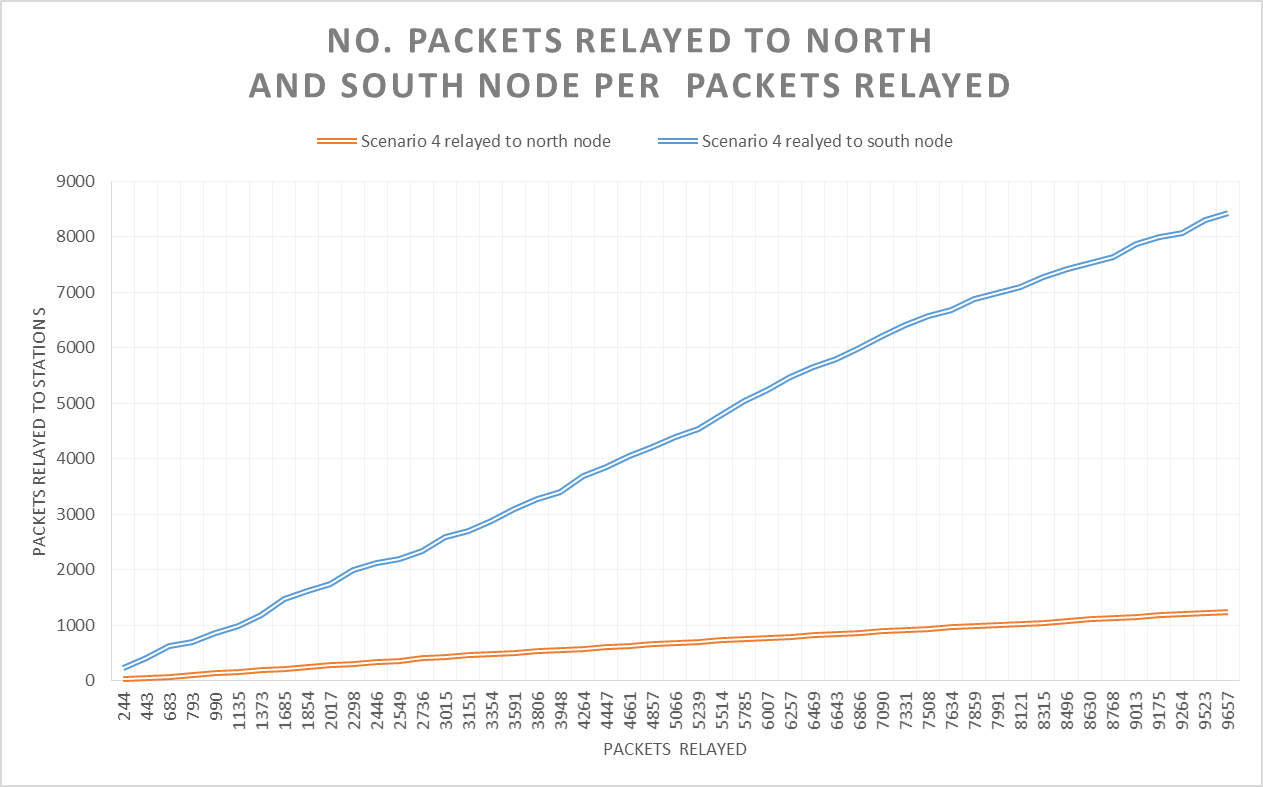
\includegraphics[width=1\linewidth]{results/NoPacketsRelayedScenario4}
	\caption{No. packets relayed to north and south node in scenario 4.}
	\label{fig:nopacketsrelayedscenario4}
\end{figure}

\noindent In terms of event quality (number of packets requested ($p_1$) vs. received ($p_5$) the different scenarios has various characteristics. A optimal scenario is one where the number of requests sent is close to the number of data packets received, that is $p_1 \approx p_5$. If $p_1$>$p_5$, we have asked for more events than received, i.e. packets have not been send or lost. If $p_1$<$p_5$, we have received more events than asked for, i.e. information overhead. Table \ref{table:eventquality} shows event quality for each scenario (1-4). We see that scenario 4 provides the overall best event quality, i.e. using a channel with less traffic and increasing the length of the track, hence relying more on the relay stations.

\begin{table}[h]
	\centering
	\begin{tabular}{|l|l|l|l|} \hline
		Scenario & \pbox{4cm}{Requests \\ sent} & \pbox{18cm}{DATA's \\ received} & \pbox{18cm}{\% Quality \\ difference.} \\ \hline
		1 & 29148 & 34167 & $17.2\%$ \\ \hline
		2 & 29838 & 23563 & $-21.0\%$ \\ \hline
		3 & 29258 & 32830 & $12.2\%$ \\ \hline
		4 & 30523 & 28874 & $-5.4\%$ \\ \hline
	\end{tabular}
	\caption{Event quality from scenarios 1-4.}
	\label{table:eventquality}
\end{table}

\noindent Looking at the energy consumption, the smaller the track the less total energy will be consumed because of less messages relayed. This result in less total energy consumed because the relays are inactive, assuming the relays are sleeping when inactive. However this is not true in the test scenarios, but in a optimized scenario this would be the case and is therefore concluded upon. Energy consumption per packet sent can be found in table \ref{table:energyConsumption}. As shown, the total energy consumption of the system as well as that of the base station itself is higher in scenario 2 and 4 because of the extra request messages send through relays. The conclusion is that the more messages or packets that needs relaying the more energy is consumed overall.

\begin{table}[H]
	\centering
	\begin{tabularx}{\linewidth}{|X|X|X|}
		\hline
		Scenario	& Total energy [Ah]	& Base station percentage used [\%]	\\ \hline
		1			& $0.577$			& $8.81$							\\ \hline
		2			& $0.731$			& $9.02$							\\ \hline
		3			& $0.581$			& $8.84$							\\ \hline
		4			& $0.632$			& $9.23$							\\ \hline
	\end{tabularx}
	\caption{Energy consumption assuming a specific cost per packet sent. "Total energy" is the energy consumed by the whole system. "Base station percentage used" is the percentage of the total energy used by the base station.}
	\label{table:energyConsumption}
\end{table}